% Especificaciones del tamaño de letra, tamaño de hoja, márgenes, librerias, etc.
\documentclass[12pt, letterpaper]{article}
\usepackage[english]{babel}
\usepackage[utf8]{inputenc}
\usepackage[T1]{fontenc}
\usepackage{amsmath}
\usepackage{graphicx}
\usepackage{subcaption}
\usepackage{hyperref}
\usepackage{url}
\usepackage{amssymb}
\usepackage{float}
\usepackage[margin=1in]{geometry}
\renewcommand{\baselinestretch}{1.5}

% Enlace Bibliografía
\usepackage{csquotes}
\usepackage[notes,backend=biber]{biblatex-chicago}
\addbibresource{referencias.bib}

% Titulo, autores, fecha.
\title{Práctica \#8: Análisis de Torsión}
\author{Carlos Vásquez 1155057}

% Inicio del documento
\begin{document}
\maketitle
\section*{Introducción}
En esta práctica nos enfocaremos en el análisis de un cilíndro al cual se le aplicará un par torsional y así calcular los esfuerzos cortantes debidos a la torsión interna que se genera en éste. Posteriormente nos aseguraremos de comprobar estos resultados mediante simulaciones en SOLIDWORKS y así cersiorarnos más de estos resultados.

\section*{Desarrollo}

Las especificaciones de la pieza se detallan a continuación, junto con el esfuerzo que se realizará sobre ella:

\textit{Determinar el máximo esfuerzo cortante en un eje de 3'' de diámetro. El par aplicado es de $36000\ lb \cdot ft$.}

Para este análisis realizamos un cilíndro sólido en SOLIDWORKS, del largo que sea (en este caso se optó por un diámetro de 5'') pero del diámetro que se especificó. El material que se aplicó al cilindro fue acero ASTM A36. Posteriormente se colocó una sujeción al cilindro como se muestra a continuación:

\begin{figure}[H]
	\centering
	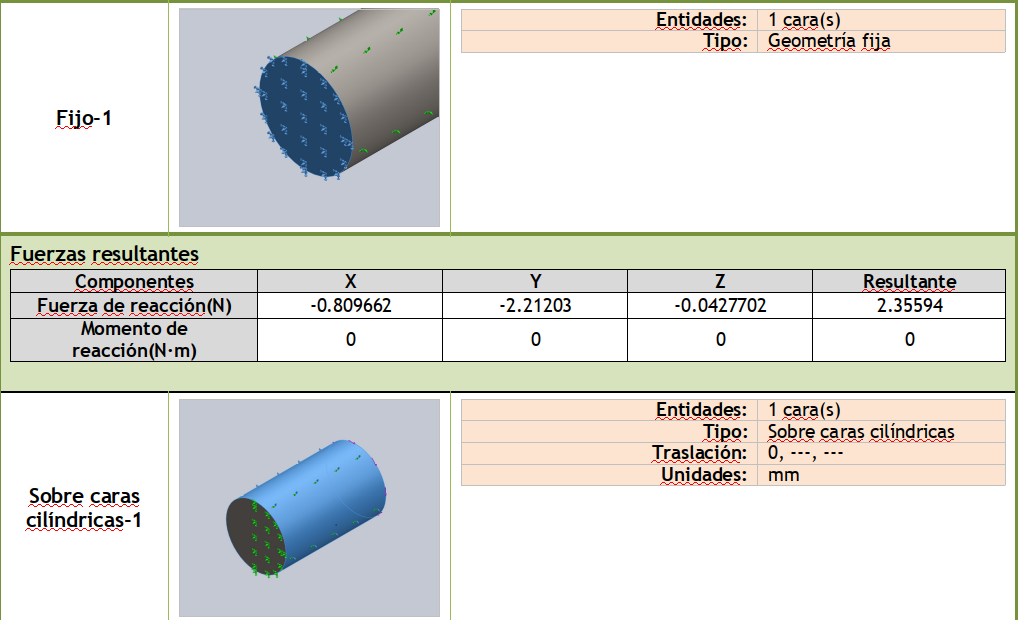
\includegraphics[width=\textwidth]{sujeciones.png}
	\caption{Sujeciones aplicadas al cuerpo.}
\end{figure}

Una vez añadida esta sujeción, se colocó el par torsional. Hecho esto también hemos agregado una malla para hacer un cálculo mediante aproximación por polígonos.

\begin{figure}[H]
	\centering
	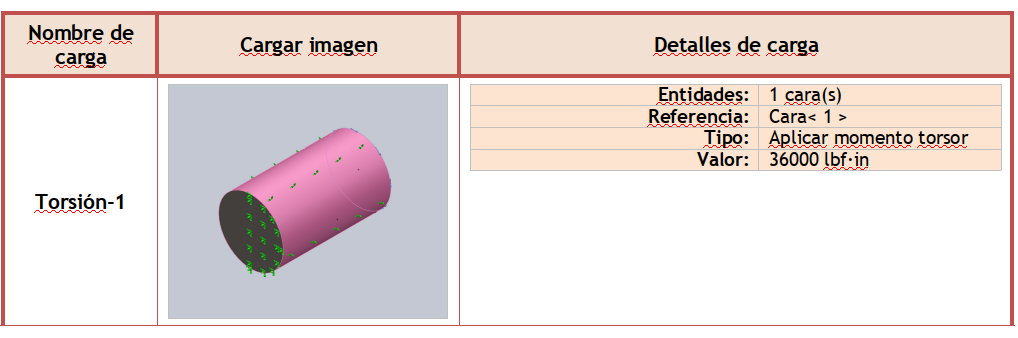
\includegraphics[width=\textwidth]{par.png}
	\caption{Par torsional de $36000\ lb \cdot ft$.}
\end{figure}

\begin{figure}[H]
	\centering
	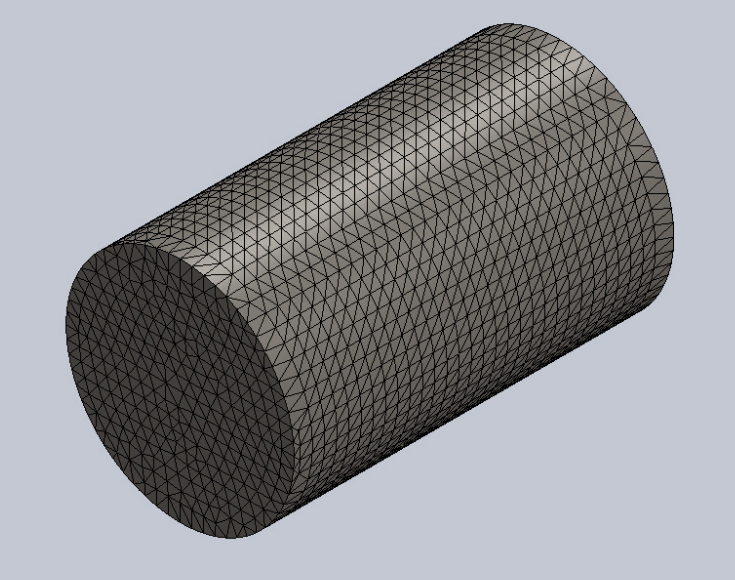
\includegraphics[width=0.7\textwidth]{malla.png}
	\caption{Malla que se añadió al sólido.}
\end{figure}

Los resultados del análisis se muestran a continuación:

\begin{figure}[H]
	\centering
	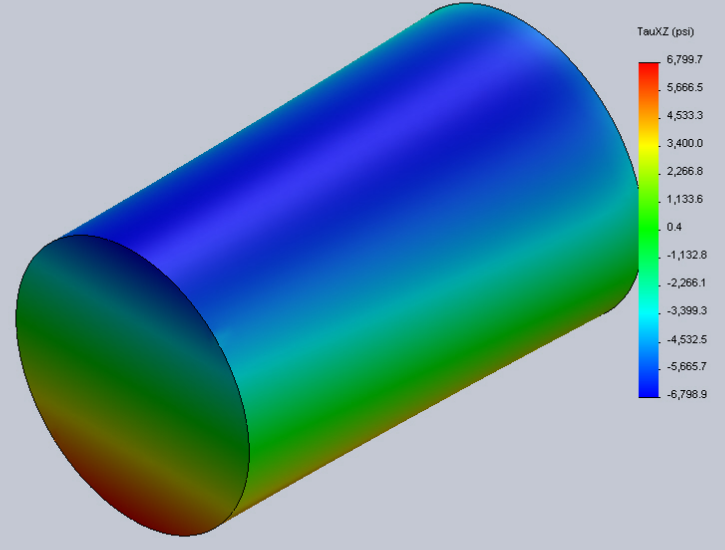
\includegraphics[width=0.7\textwidth]{data.png}
	\caption{Resultados de la simulación.}
\end{figure}

\section*{Cálculos}

Para realizar este ejercicio partimos de las siguientes fórmulas necesarias para calcular lo que se nos pide.

\begin{equation}
	J = \frac{\pi D^4}{32}
\end{equation}

\begin{equation}
	\tau_{max} = \frac{Tc}{J}
\end{equation}

Donde la eq. (1) es el momento polar de inercia con el que cuenta nuestro cilíndro y la eq. (2) es el máximo esfuerzo que experimentará nuestra barra cilíndrica.

Dados los datos, calculamos el momento polar de torsión primeramente:

\begin{equation}
	\begin{split}
		J &= \frac{\pi (3\ in)^4}{32}\\
		J &= 7.95\ in^4
	\end{split}
\end{equation}

Ahora que contamos con el momento polar de inercia podemos calcular el esfuerzo máximo que sufrirá el eje.

\begin{equation}
	\boxed{\begin{split}
		\tau_{max} &= \frac{(36000\ lb \cdot ft)(1.5\ in)}{7.95\ in^4}\\
		\tau_{max} &= 6792.45\ \frac{lb}{in^2}
	\end{split}}
\end{equation}
\section*{Conclusión}

Al observar los resultados de la simulación en SOLIDWORKS y los resultados de los cálculos teóricos podemos concluir que ambos son bastante cercanos. Lo único que es un poco distinto de lo idealizado es el campo vectorial del esfuerzo que se presenta en el análisis de la simulación. La figura debería de mostrar un mayor esfuerzo mientras más lejana es la distancia del centro. Por este motivo, la superficie debería de estar completamente rojiza y el centro relativamente azul, en especial en el centro.
%%%%%  Bib
\renewcommand\refname{Referencias}
\printbibliography
\end{document}
